\documentclass[journal]{IEEEtran}
\usepackage{cite}
\usepackage{amsmath,amssymb,amsfonts}
\usepackage{graphicx}
\usepackage{textcomp}
\usepackage{xcolor}
\usepackage{hyperref}
\usepackage{algorithm}
\usepackage{algpseudocode}

\hypersetup{
    colorlinks=true,
    linkcolor=blue,
    filecolor=magenta,      
    urlcolor=cyan,
}

\begin{document}

\title{Dynamic Hybrid Forecasting Models for Drug Consumption Prediction in Hospital Pharmacies}

\author{Yuxin Fan$^{*}$ and Siye Wu$^{\dagger}$ \\
$^{*}$School of Engineering and Applied Science, University of Pennsylvania, Canada, Toronto \\
Email: yuxinfan@alumni.upenn.edu \\
$^{\dagger}$Simon Business School, University of Rochester, Canada, Toronto \\
Email: april.siyewu@hotmail.com}

\maketitle

\begin{abstract}
Accurate and efficient drug consumption forecasting is crucial for hospital pharmacies to avoid overstocking, minimize wastage, and ensure continuous patient care. This study proposes a hybrid forecasting framework integrating XGBoost, Prophet, and SARIMAX to improve monthly consumption predictions at the drug-manufacturer level. Through rolling-window forecasting and advanced feature engineering, the proposed approach addresses challenges such as seasonality, trend shifts, and sparse data. Experimental results demonstrate significant improvements in prediction accuracy and robustness across diverse drug consumption scenarios.
\end{abstract}

\begin{IEEEkeywords}
Drug Consumption Forecasting, Hospital Pharmacies, Forecasting Models, XGBoost, Prophet, SARIMAX
\end{IEEEkeywords}

\section{Introduction}

Drug consumption forecasting plays a critical role in hospital pharmacy inventory management. Accurate drug consumption predictions enable hospital pharmacies to ensure drug availability while minimizing costs associated with overstocking or stockouts. As highlighted by Koala et al.~\cite{koala2021factors}, forecasting drug consumption is particularly challenging due to numerous influencing factors, such as sociodemographic characteristics, morbidity patterns, drug price index, and seasonal factors like disease outbreaks or policy changes, resulting in highly complex and dynamic consumption patterns. Therefore, the purpose of our study is to integrate a hybrid framework combining machine learning and statistical models to enhance drug consumption forecasting for hospital pharmacies.

In previous studies, various forecasting techniques have been proposed to address one or more of the above challenges. For instance, Taylor and Letham~\cite{taylor2018forecasting} introduced Prophet, a scalable forecasting method designed for large-scale applications, which excels at capturing general trends and seasonality through changepoint detection. However, Prophet often requires careful tuning to prevent overfitting to localized patterns and has limited capability in incorporating external variables, which are critical in drug consumption forecasting due to the influence of factors such as pricing and policies. Extreme Gradient Boosting (XGBoost), proposed by Chen and Guestrin~\cite{chen2016xgboost}, has demonstrated remarkable success in applications such as sales prediction and customer behavior modeling, highlighting its flexibility across diverse domains. However, XGBoost struggles with sequential dependencies in time-series data, making it less effective in forecasting tasks where temporal order plays a critical role, such as tracking drug consumption patterns over time.

The above limitations highlight a common challenge of single-model approaches, which often struggle to generalize across datasets exhibiting varying seasonality, non-linear dependencies, and sparsity. Therefore, some hybrid model frameworks have been introduced to provide more robust solutions. Comparative studies like those by Meng et al.~\cite{meng2021comparative} highlight that while Long Short-Term Memory (LSTM) demonstrates superior accuracy in drug sales forecasting, due to its ability to capture long-term dependencies and non-linear patterns, Prophet remains an effective tool for handling time series data with seasonality and holiday effects. However, both models exhibit limitations, such as LSTM's higher computational requirements and Prophet's sensitivity to trend and seasonality assumptions, which may hinder their adaptability in scenarios where drug consumption is influenced by dynamic external factors like policy changes or sudden disease outbreaks. Xu et al.~\cite{xu2019hybrid} propose a hybrid approach that combines a linear regression (LR) model, specifically the auto-regression (AR) or auto-regressive integrated moving average (ARIMA) model, and a deep belief network (DBN) to improve time series forecasting by capturing both linear and nonlinear patterns. While this method demonstrates high accuracy in general time series prediction, its reliance on computationally intensive DBN training and limited consideration of irregular external factors, may pose challenges in hospital pharmacy drug consumption forecasting. Siddiqui et al.~\cite{siddiqui2021hybrid} propose a hybrid forecasting model, ARIMA-Holt’s Winter (ARHOW), which combines the strengths of the ARIMA model and the Holt-Winters method to enhance forecasting accuracy. This study, specifically applied to the pharmaceutical industry, demonstrates that this hybrid model involves high demand volatility and complex seasonal patterns. However, the reliance on fixed model architectures and pre-determined parameter settings may limit its adaptability in highly dynamic environments. Rathipriya et al.~\cite{rathipriya2022pharma} develop a hybrid demand forecasting model using both shallow neural networks like Radial Basis Function Neural Network (RBF\_NN) and Generalized Regression Neural Network (GR\_NN), and deep learning models like LSTM and Stacked LSTM to predict pharmaceutical sales. Their study highlights the effectiveness of shallow neural networks in handling smaller datasets and mitigating noise, while deep learning models like LSTM excel at capturing non-linear and temporal patterns in larger datasets. However, the computational complexity of deep learning models and their dependency on large datasets may pose challenges in hospital pharmacy drug consumption forecasting, where data sparsity and rapid external changes often occur.

In this study, to address the limitations of existing models, such as adjusting predictions for non-stationary data, capturing shifting trends dynamically, and accounting for diverse drug-manufacturer combinations, our proposed framework introduces a new hybrid model called DynamicXSP integrating XGBoost, Prophet, and Seasonal AutoRegressive Integrated Moving Average with eXogenous variables (SARIMAX) with rolling-window forecasting, advanced feature engineering and grid search. The dataset used for this study includes monthly drug consumption records collected from hospital pharmacies over a period of nearly seven years, including a wide variety of drugs and manufacturers. Models in DynamicXSP like Prophet excel at capturing stable long-term trends and seasonal patterns, making them suitable for drugs with high and regular demand. On the other hand, SARIMAX is better equipped to handle datasets influenced by external variables or strong short-term dynamics, as it integrates advanced feature engineering and external factor modeling. For scenarios with complex non-linear relationships or sparse observations, XGBoost proves advantageous due to its flexibility in handling feature interactions and non-linear dependencies. Therefore, DynamicXSP enriches the data with lag features and trend indicators, capturing both short-term dependencies and long-term dynamics. This synergy provides a robust and versatile solution to the unique challenges of drug consumption forecasting, making the framework applicable across various drug types and manufacturers.

The remainder of this paper is organized as follows: Section II details the methodology, highlighting the advantages of the proposed framework. Section III presents experimental and results, including data preprocessing and data analysis. Finally, Section IV concludes the study and outlines future research directions.

\section{Methodology}

\subsection{DynamicXSP Model Framework}

[probably can remove] The proposed hybrid forecasting framework integrates the complementary strengths of Prophet, SARIMAX, and XGBoost to address the diverse challenges in drug consumption prediction.

Drug consumption data exhibits significant variability, with some combinations showing consistent trends while others experience volatility or irregular demand. 

To optimize predictions, the framework dynamically selects the most appropriate model for each drug-manufacturer combination. Performance metrics such as R\(^2\) and symmetric mean absolute percentage error (SMAPE) are employed to evaluate each model’s effectiveness. With a high R\(^2\) score and low SMAPE [indicates that the model captures most of the variance in the data, while a low SMAPE value reflects accuracy in representing relative changes.] This data-driven model selection process ensures that the framework adapts to heterogeneous consumption patterns, maximizing prediction accuracy and robustness.

[remove] By dynamically assigning models based on their strengths, the hybrid framework efficiently handles diverse scenarios. Prophet is ideal for stable and predictable datasets, SARIMAX excels in addressing external factors and seasonality, while XGBoost captures non-linear and sparse patterns. This synergy of models enhances the overall robustness of the forecasting system, providing a scalable and versatile solution for hospital pharmacies managing a wide range of drug consumption trends.

\subsection{Model Design and Roles}
\subsubsection{DynamicXSP-S (SARIMAX) Model}

SARIMAX extends the traditional ARIMA model by incorporating external (exogenous) variables, making it well-suited for time-series data with seasonality, trends, and contextual factors. The model is defined as:

\begin{equation}
y_{t} = \phi(B)\theta(B)^{-1} \left( c + \mathbf{X}_{t}\beta + \epsilon_{t} \right),
\end{equation}

where \(y_{t}\) represents the target variable (e.g., monthly drug consumption), \(\mathbf{X}_{t}\) denotes the exogenous variables, and \(\epsilon_{t}\) is the white noise error term. 

To enhance prediction accuracy, our SARIMAX utilizes advanced feature engineering to incorporate exogenous variables, including:

\begin{itemize}
    \item \textbf{Lagged values}: Capture delayed effects of past consumption:
    \begin{equation}
    \text{lag}_{k} = y_{t-k}, \quad k \in \{1, 3, 6, 12\}.
    \end{equation}
    
    \item \textbf{Rolling statistics}: Represent short-term trends and variability:
    \begin{align}
    \text{Rolling Mean}_{k} &= \frac{1}{k} \sum_{i=1}^{k} y_{t-i}, \\
    \text{Rolling Std}_{k} &= \sqrt{\frac{1}{k} \sum_{i=1}^{k} (y_{t-i} - \text{Mean})^2}.
    \end{align}
    
    \item \textbf{Seasonality}: Encode monthly seasonality using trigonometric functions:
    \begin{align}
    \text{Month\_sin} &= \sin\left(\frac{2\pi \cdot \text{Month}}{12}\right), \\
    \text{Month\_cos} &= \cos\left(\frac{2\pi \cdot \text{Month}}{12}\right).
    \end{align}
    
    \item \textbf{Exponential weighted moving average (EWMA)}: Smoothing recent observations:
    \begin{equation}
    \text{EWMA}_{\alpha} = \alpha y_{t} + (1-\alpha) \cdot \text{EWMA}_{\alpha,t-1}.
    \end{equation}
    
    \item \textbf{Percentage change and trend strength}: Capture relative variations and long-term dynamics:
    \begin{align}
    \text{Pet\_Change}_{k} &= \frac{y_{t} - y_{t-k}}{y_{t-k}}, \\
    \text{Trend Strength} &= \frac{1}{k} \sum_{i=1}^{k} \lvert y_{t-i} - y_{t-i-1} \rvert.
    \end{align}
\end{itemize}

These engineered features enable SARIMAX to capture both short-term dependencies and long-term trends, significantly enhancing its ability to model complex temporal patterns in drug consumption data.

\subsubsection{DynamicXSP-X (XGBoost) Model}

XGBoost is a gradient boosting framework that constructs an ensemble of decision trees to predict the target variable \(y_t\). It is particularly effective for time-series forecasting involving non-linear relationships and sparse data. The model predicts \(y_t\) through an additive function:

\begin{equation}
\hat{y}_{t} = F(x_{t}) = \sum_{k=1}^{K} f_{k}(x_{t}), \quad f_{k} \in \mathcal{F},
\end{equation}

where \(\hat{y}_{t}\) is the predicted value, \(x_{t}\) represents input features, \(f_{k}\) denotes the \(k\)-th decision tree, and \(\mathcal{F}\) is the space of decision trees.

\textbf{Feature Engineering:} Temporal dependencies are captured using lagged values (\(y_{t-1}, y_{t-2}, \dots\)), rolling statistics (e.g., moving averages and standard deviations over 3, 6, and 12 periods), and seasonal patterns encoded via trigonometric functions (\(\sin, \cos\)). Interaction terms between lagged values and seasonal indicators further enhance the model's ability to capture complex dependencies.

\textbf{Rolling-Window Training:} The model employs a rolling-window approach to dynamically adapt to evolving trends. At each iteration, the training dataset is updated with the most recent observations, and the model is retrained to make predictions for the next time step, ensuring adaptability and minimizing overfitting.

\textbf{Hyperparameter Optimization:} To maximize performance, a grid search tunes parameters such as:
\begin{itemize}
    \item \textit{Number of estimators}: Determines ensemble size.
    \item \textit{Learning rate}: Controls the contribution of each tree.
    \item \textit{Maximum tree depth}: Prevents overfitting by limiting tree complexity.
    \item \textit{Subsample and column sampling ratios}: Enhance generalization by regulating data and feature subsets.
\end{itemize}

By modeling non-linear interactions and addressing irregular patterns, XGBoost complements statistical models like SARIMAX. Its integration with rolling-window training and advanced feature engineering ensures robust and adaptive predictions, making it a key component of the hybrid forecasting framework.


\subsubsection{DynamicXSP-P (Prophet) Model}

Prophet is a time-series forecasting model developed by Facebook, designed to decompose data into trend, seasonality, and holiday components. It is particularly effective in handling missing values, outliers, and irregular patterns, making it suitable for dynamic drug consumption data. The model predicts the target variable \(y_t\) as:

\begin{equation}
y_{t} = g(t) + s(t) + h(t) + \epsilon_{t},
\end{equation}

where \(g(t)\) represents the long-term trend, \(s(t)\) captures seasonal patterns using Fourier series, \(h(t)\) accounts for holiday effects, and \(\epsilon_{t}\) is the white noise error term. This decomposition enhances interpretability while maintaining predictive accuracy.

\textbf{Hyperparameter Optimization:} Key hyperparameters are optimized via grid search:
\begin{itemize}
    \item \textit{seasonality\_mode}: Models seasonal effects as additive or multiplicative.
    \item \textit{changepoint\_prior\_scale}: Controls flexibility for abrupt trend changes.
    \item \textit{seasonality\_prior\_scale}: Adjusts the weight of seasonal components.
\end{itemize}
A higher \textit{changepoint\_prior\_scale} enables the model to adapt to frequent structural changes, while lower values favor smoother transitions.

\textbf{Rolling-Window Forecasting:} The model employs a rolling-window strategy, retraining on the most recent data at each iteration. This ensures adaptability to emerging trends while mitigating the impact of outdated patterns, making it robust for datasets with irregular or sparse observations.

By combining decomposition capabilities, grid search optimization, and rolling-window forecasting, Prophet provides accurate and interpretable predictions, complementing the other components of the hybrid framework.

\subsection{Dynamic Rolling-Window Forecasting}

Time-series data often exhibit non-stationarity, where trends, seasonality, and noise evolve over time. Static forecasting approaches relying on fixed historical data may struggle to capture these dynamics, leading to suboptimal performance. To address this, a dynamic rolling-window forecasting strategy is employed, enabling models to prioritize recent information and adapt to structural changes.

At each time step \(t\), the training dataset is updated to include the most recent observations while discarding older data beyond the defined window size (\(W\)). Formally, the training dataset at \(t\) is defined as:

\[
\mathcal{D}_{t} = \{(y_{\tau}, \mathbf{X}_{\tau}) \mid \tau \in [t - W, t-1]\},
\]

where \(\mathcal{D}_{t}\) is the training data, \(y_{\tau}\) denotes the target variable, and \(\mathbf{X}_{\tau}\) represents feature vectors. After training on \(\mathcal{D}_{t}\), predictions are generated for the next time step (\(t+1\)).

The rolling-window approach effectively captures short-term dynamics by prioritizing recent patterns while mitigating the influence of outdated data. It is particularly advantageous for handling structural changes such as shifts in trends or seasonality. The choice of window size (\(W\)) is critical: larger windows incorporate long-term patterns, while smaller windows emphasize recent changes. This study evaluates multiple window sizes and selects the optimal configuration based on metrics such as root mean squared error (RMSE) and symmetric mean absolute percentage error (SMAPE).

Integrating rolling-window forecasting into the hybrid framework enhances adaptability:
\begin{itemize}
    \item \textbf{SARIMAX}: Dynamically recalibrates coefficients to model short-term dependencies and external influences.
    \item \textbf{XGBoost}: Refines decision trees with updated feature interactions, capturing evolving non-linear relationships.
    \item \textbf{Prophet}: Updates its trend decomposition to align with the latest data.
\end{itemize}

This iterative strategy ensures the models remain responsive and resilient to changes, achieving superior performance across diverse drug consumption scenarios by continuously adapting to the most recent dynamics.

\section{Experiments}

\subsection{Dataset}
The dataset used in this study consists of monthly drug consumption records collected from various hospital pharmacies between January 1, 2018, and September 1, 2024. The data include a diverse range of drugs across multiple categories and manufacturers, ensuring a comprehensive representation of pharmaceutical demand. Each record contains the drug name, manufacturer, monthly consumption values, inventory levels, and associated features such as proportions and trends. This dataset provides a robust foundation for developing and testing the proposed forecasting framework.

\subsection{Data Pre-processing}
A comprehensive preprocessing pipeline was applied to ensure data quality and consistency, while focusing on key steps relevant to our framework. Missing values in critical features were interpolated where possible, and records with excessive missing data were excluded to maintain dataset integrity.

[name/specify the method of outliers] Outliers in consumption data were addressed using a rolling-window approach. For each drug-manufacturer combination, rolling statistics such as mean and standard deviation were computed over a seven-month window. Values exceeding three standard deviations from the mean or falling outside the 5th and 95th percentiles were flagged as anomalies and adjusted to boundary values to preserve the time series' continuity.

To ensure the dataset included only high-quality samples for modeling, groups with fewer than six months of non-zero consumption data or those exhibiting extreme sparsity were excluded. Temporal autocorrelation of consumption data was assessed, and groups failing to exhibit sufficient autocorrelation were removed. Additional filtering criteria included variance thresholds and limits on skewness to avoid heavily imbalanced target distributions.

Feature engineering was performed to enhance the dataset's predictive power. Derived features such as lagged consumption values (e.g., previous month’s consumption), rolling statistics (e.g., mean, variance, and percent changes), and seasonality indicators encoded with trigonometric functions were created to capture temporal dependencies and periodic trends. These steps ensured that the final dataset was robust, informative, and well-suited for downstream predictive modeling tasks.

\subsection{Data Analysis}

To improve the effectiveness of forecasting models on drug consumptions, we implemented DynamicXSP model framework. Each model in Dynameic was applied to forecast sales data for a diverse set of drugs and manufacturers. The dataset consisted of weekly time series data spanning seven years, capturing trends, seasonality, and irregular fluctuations in drug consumptions. The selection of the optimal model in DynamicXSP for each drug-manufacturer pair was based on achieving the highest $R^2$ and minimizing SMAPE. 

\subsection{Model Results}
\subsubsection{Representative Drug Cases}

\paragraph{DynamicXSP-X (XGBoost) Model} % 确保 XGBoost、Prophet 和 SARIMAX 平行
\begin{itemize}
\item \textbf{Drug:} Mycophenolate Sodium Enteric Tablets
\begin{itemize}
\item \textbf{Manufacturer:} Novartis Switzerland
\item \textbf{Metrics:} $R^2 = 0.8154$, SMAPE = 25.40
\end{itemize}
XGBoost showed exceptional performance for this drug by effectively capturing the complex non-linear patterns and sudden changes in demand, particularly evident in the volatile periods of 2023-2024.
\begin{figure}[H]
\centering
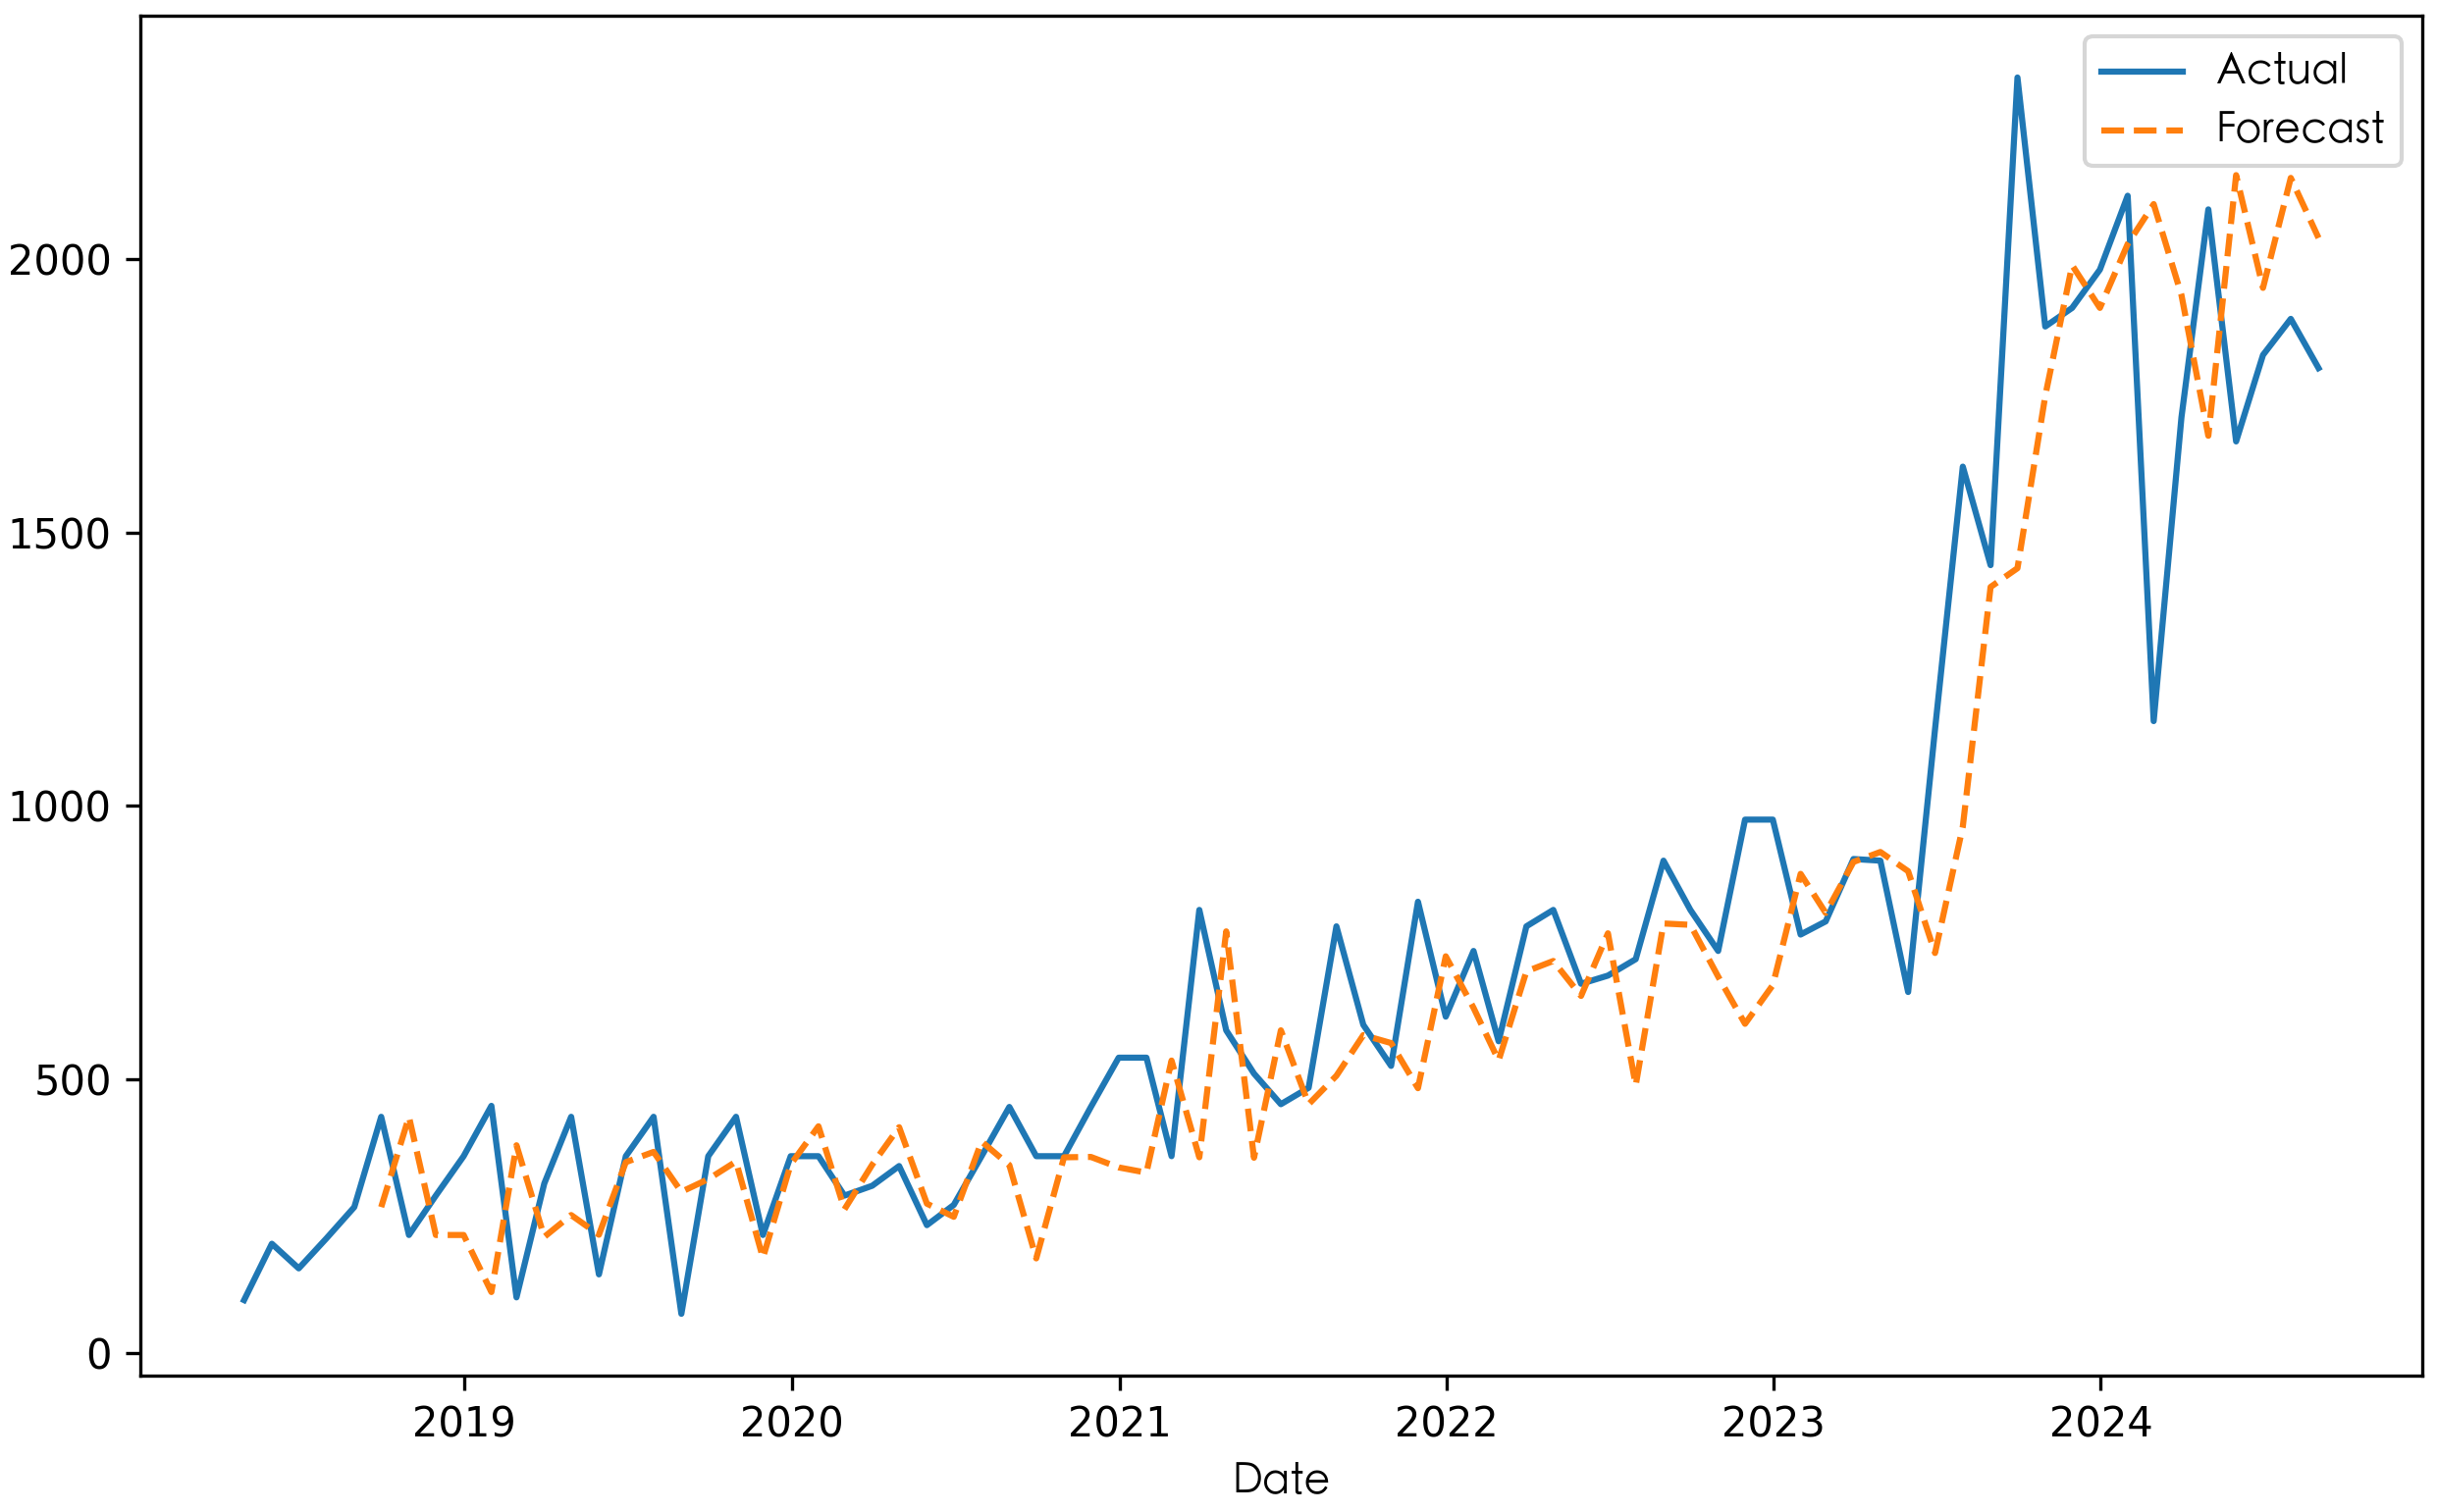
\includegraphics[width=\linewidth]{../Result_Paper/XGBoost_Prediction_麦考酚钠肠溶片_瑞士诺华.png}
\caption{XGBoost Prediction for Mycophenolate Sodium Enteric Tablets by Novartis.}
\label{fig:mycophenolate}
\end{figure}
\item \textbf{Drug:} Flurbiprofen Gel Patch
\begin{itemize}
\item \textbf{Manufacturer:} Jingtaide
\item \textbf{Metrics:} $R^2 = 0.7902$, SMAPE = 21.14
\end{itemize}
XGBoost effectively handled the increasing trend and high volatility in sales, demonstrating its strength in capturing complex patterns and sudden market changes.
\begin{figure}[H]
\centering
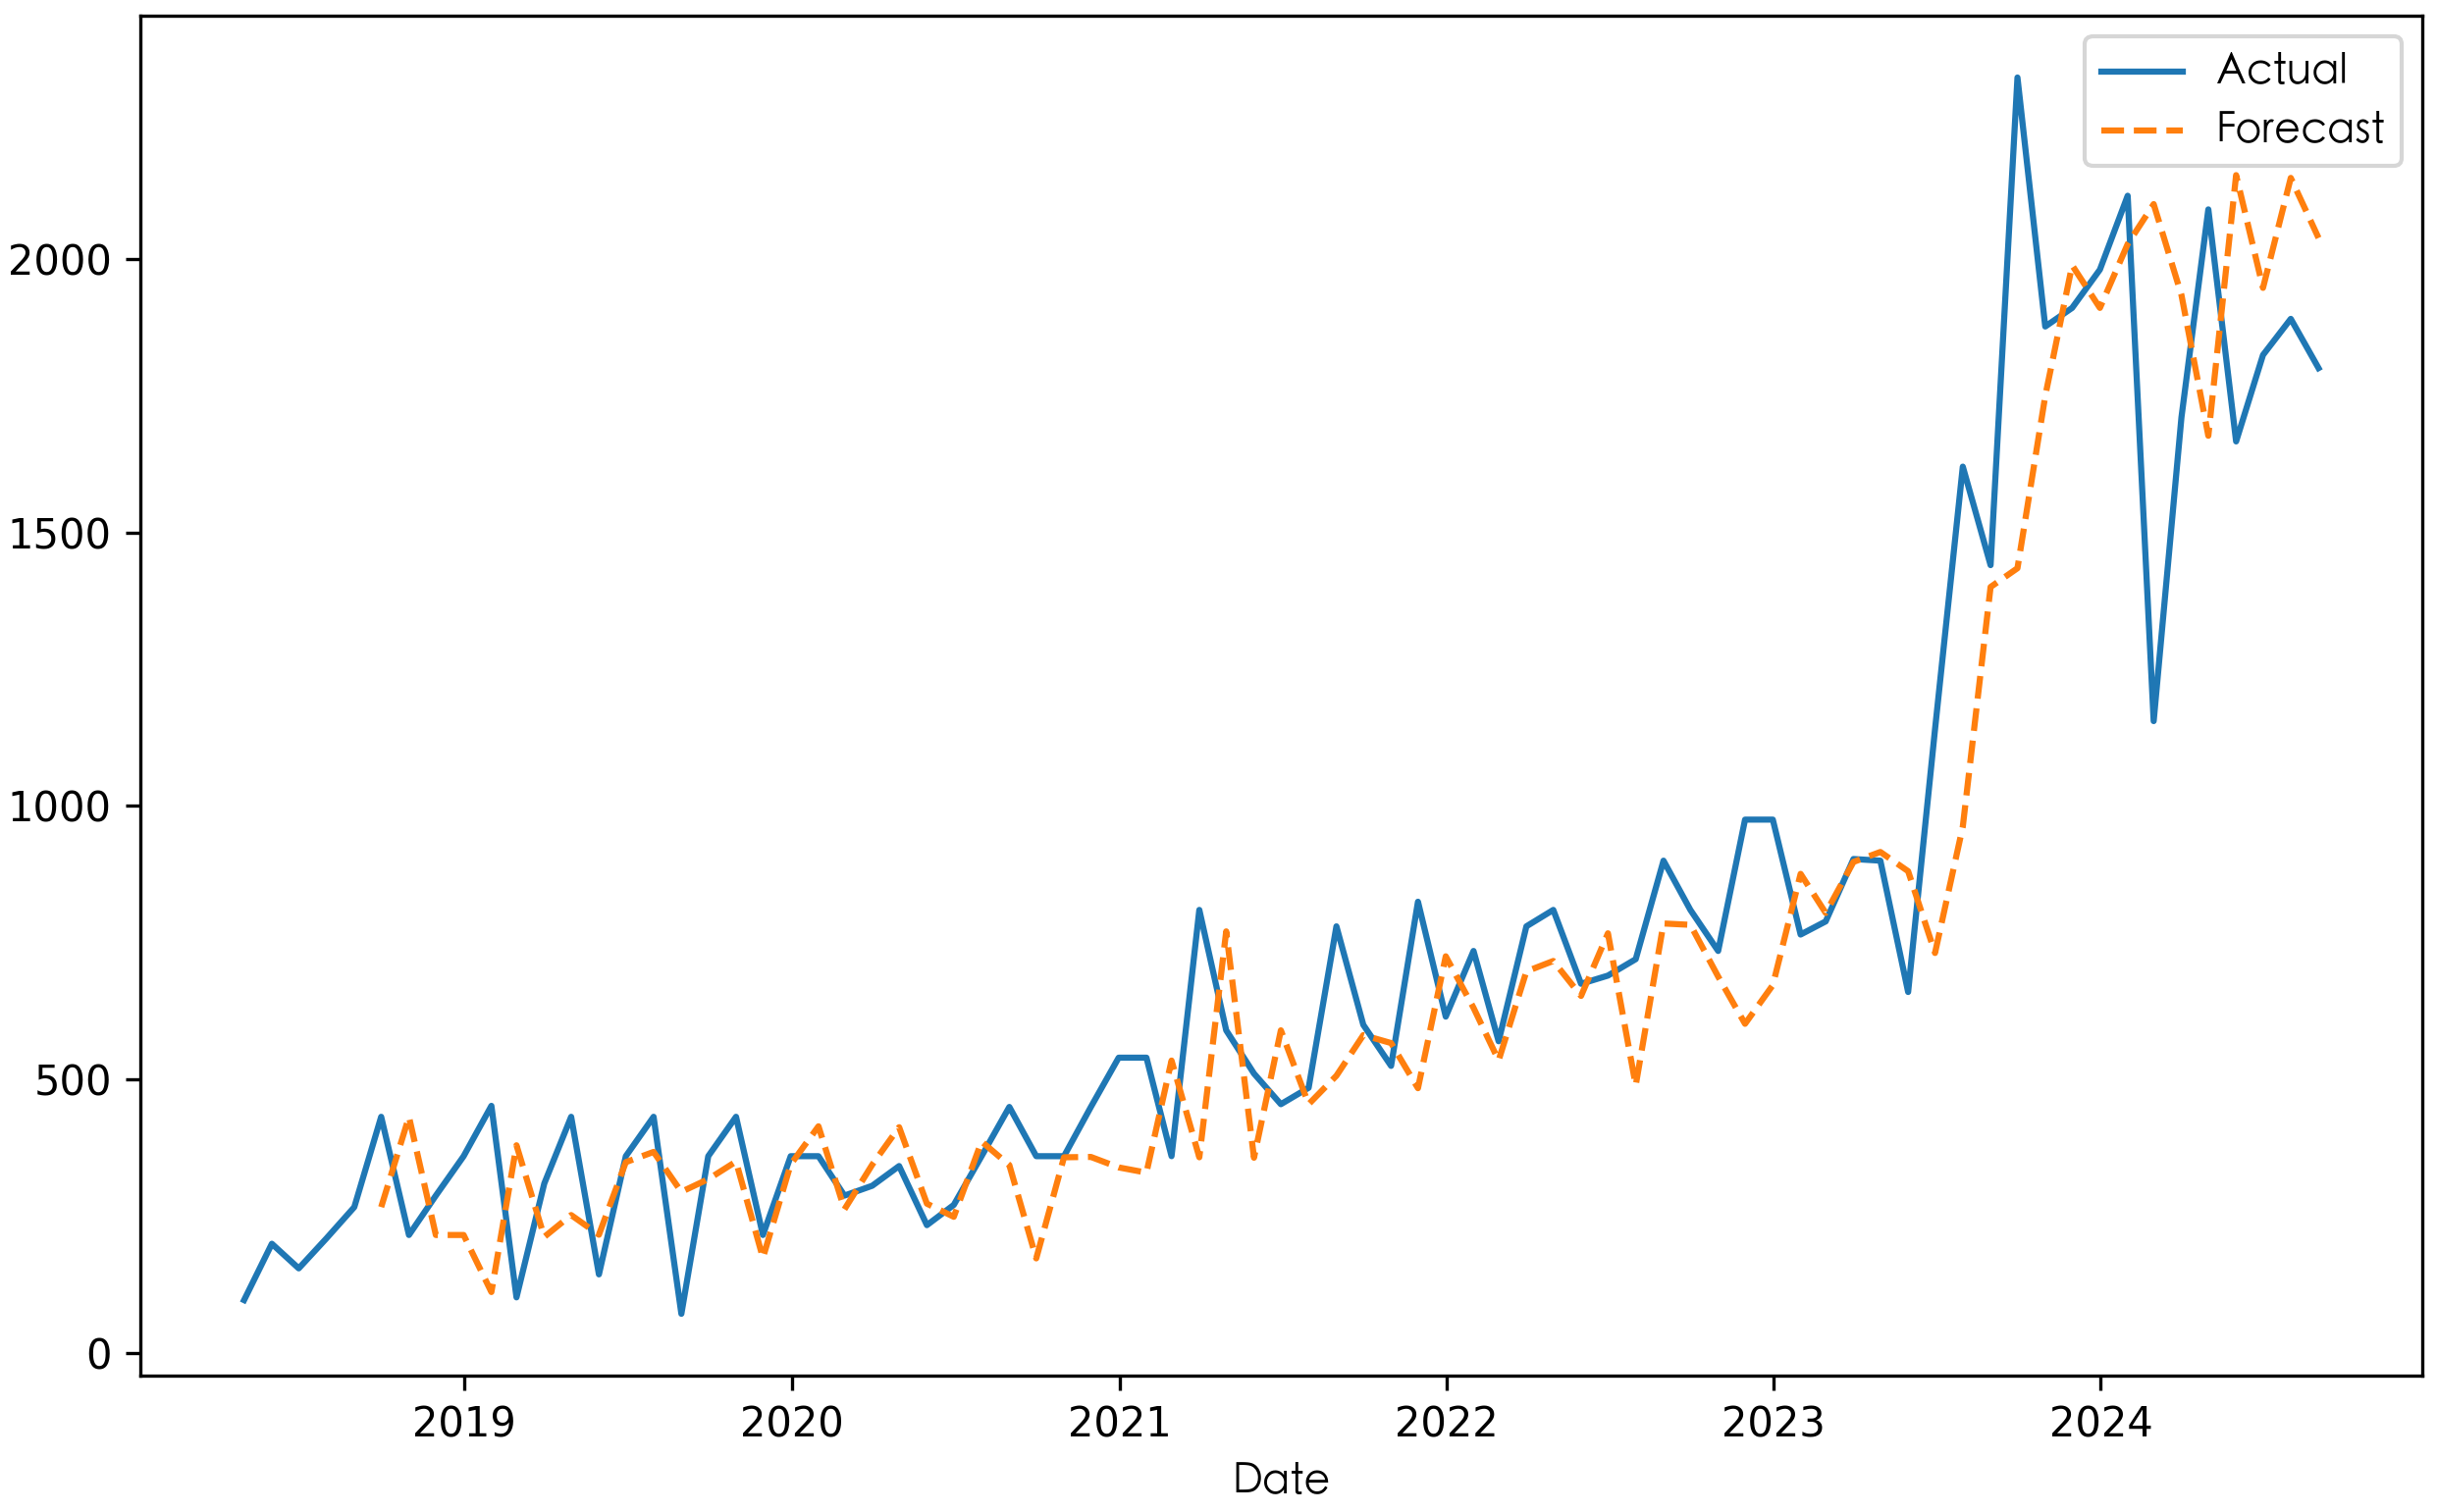
\includegraphics[width=\linewidth]{../Result_Paper/XGBoost_Prediction_麦考酚钠肠溶片_瑞士诺华.png}
\caption{XGBoost Prediction for Flurbiprofen Gel Patch by Jingtaide.}
\label{fig:flurbiprofen}
\end{figure}
\end{itemize}

\paragraph{DynamicXSP-P (Prophet) Model}
\begin{itemize}
\item \textbf{Drug:} Compound Phellodendron Liquid
\begin{itemize}
\item \textbf{Manufacturer:} Lu Hanfang
\item \textbf{Metrics:} $R^2 = 0.7898$, SMAPE = 22.63
\end{itemize}
Prophet excelled in modeling this drug's sales pattern due to its robust handling of trend changes and seasonal variations, particularly evident in the steady growth pattern.
\begin{figure}[H]
\centering
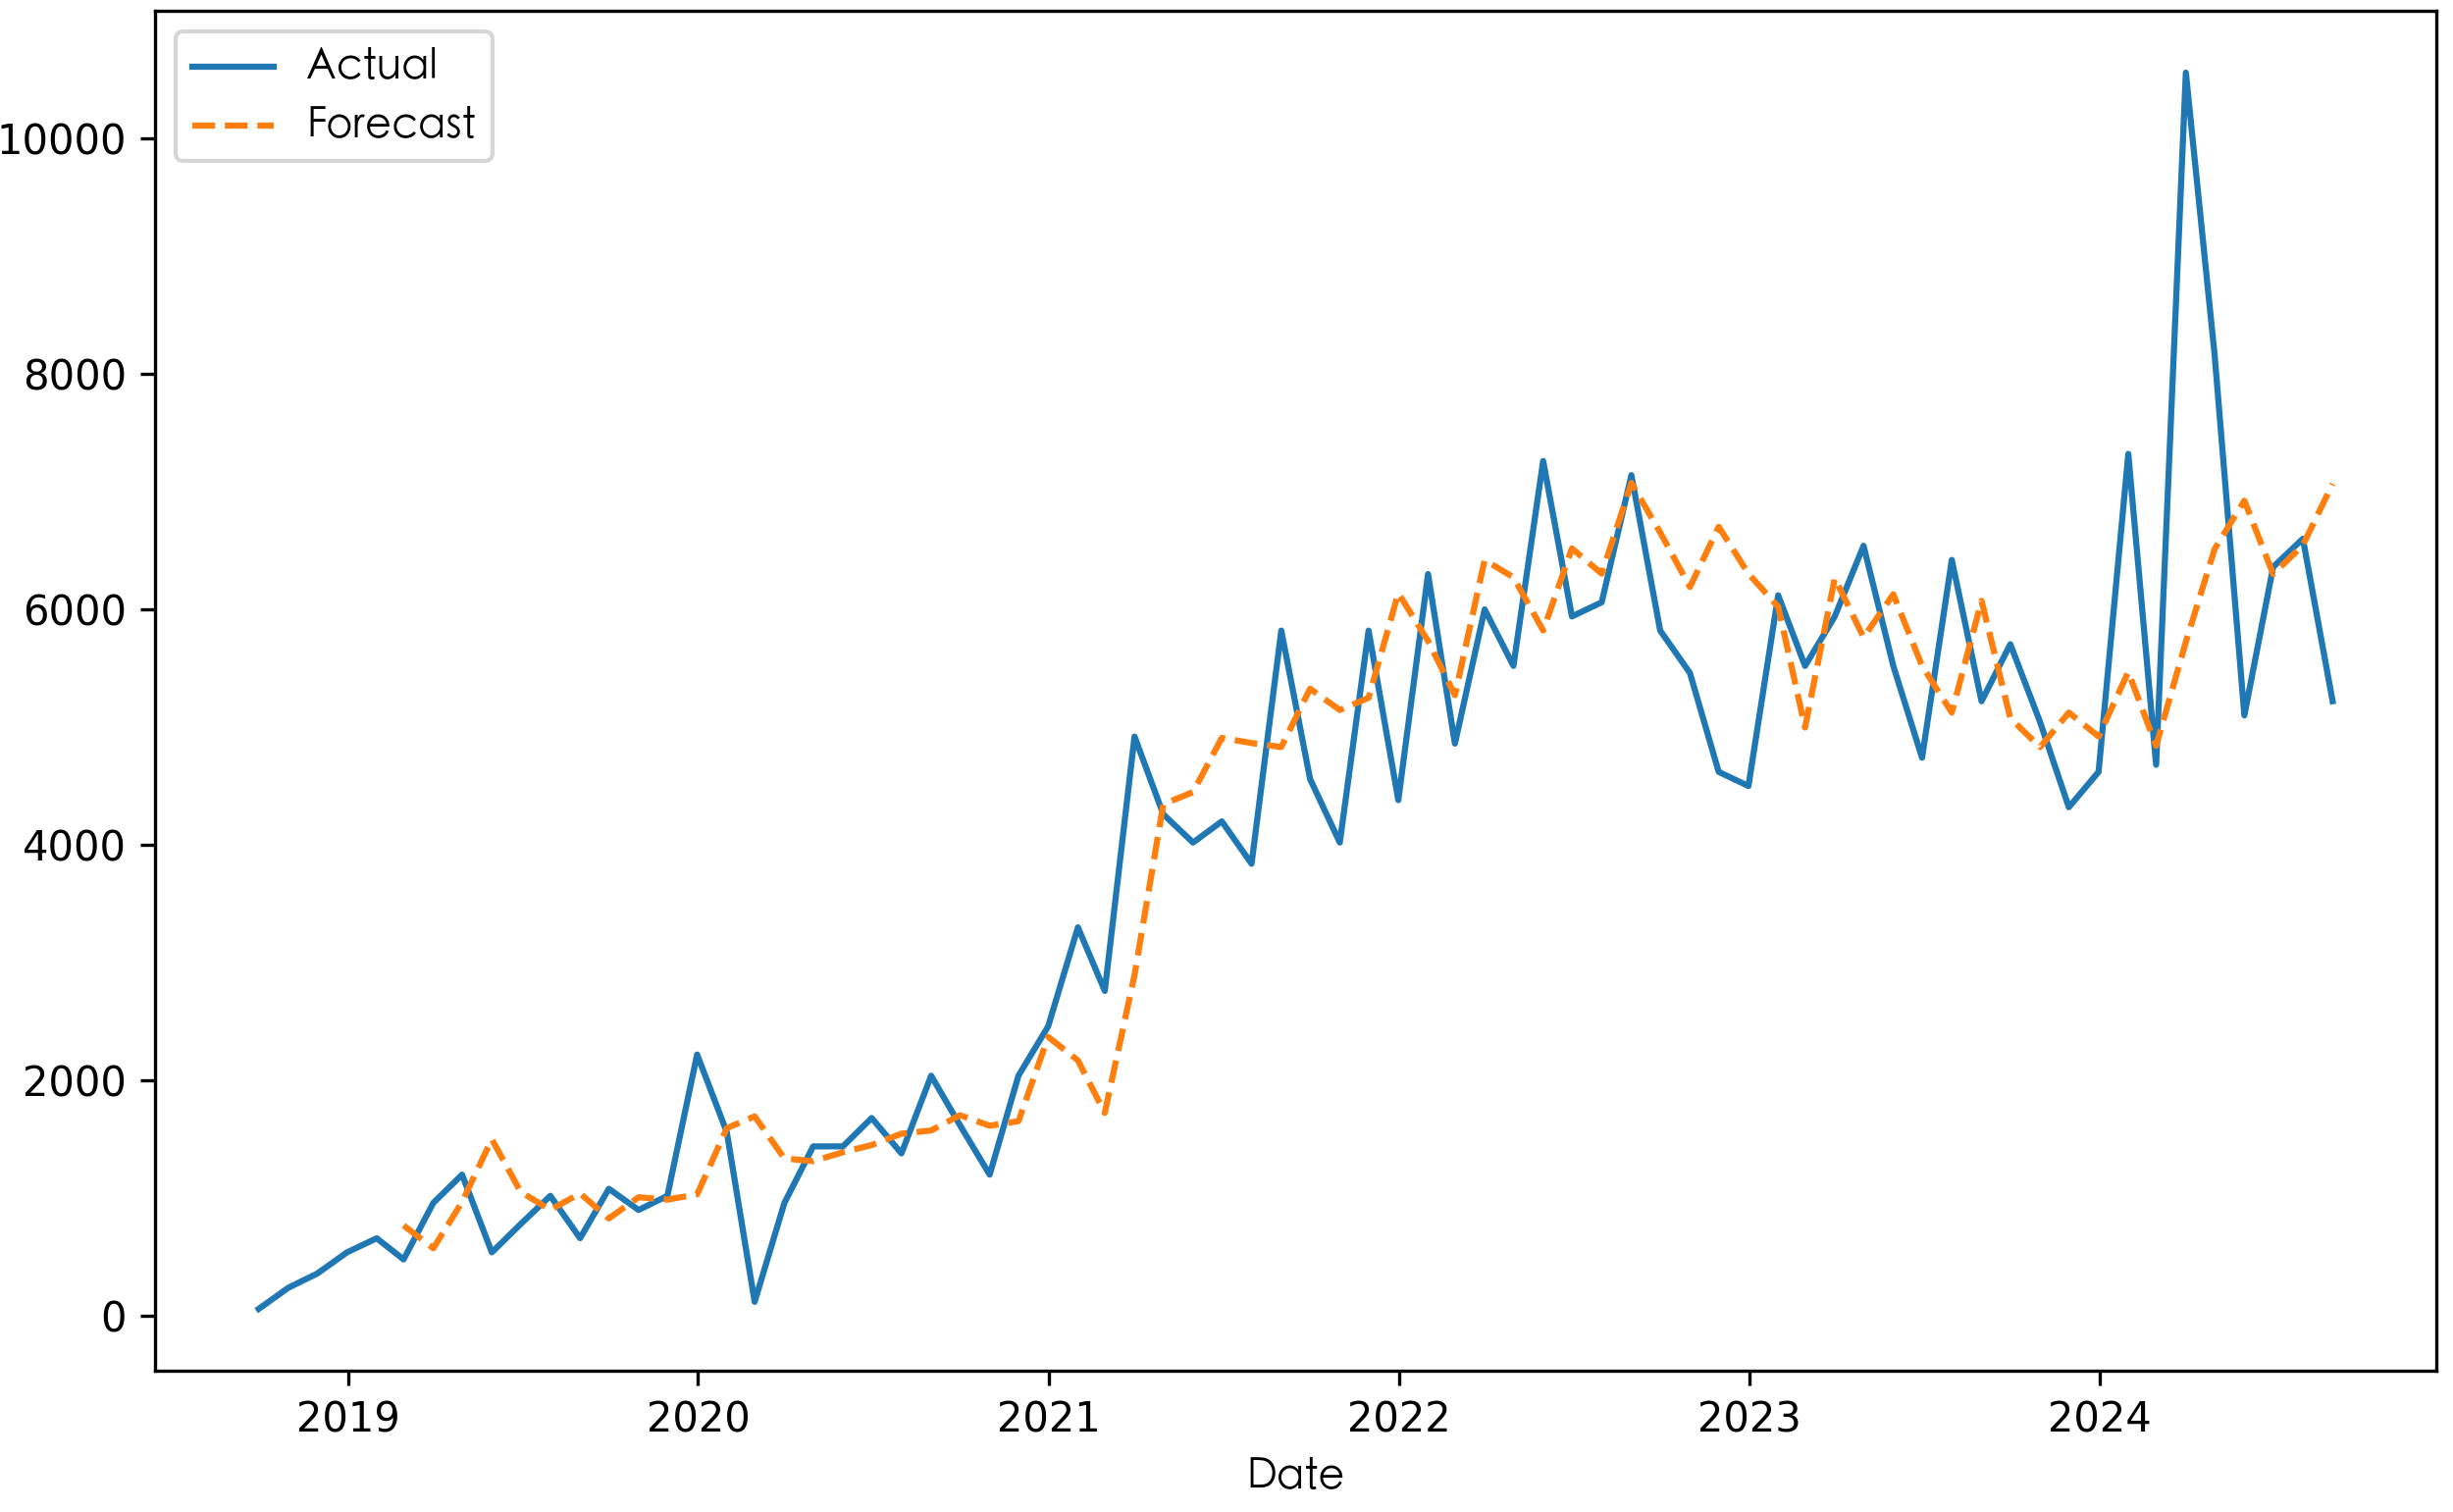
\includegraphics[width=\linewidth]{../Result_Paper/Prophet_Prediction_复方黄柏液涂剂_鲁汉方.png}
\caption{Prophet Prediction for Compound Phellodendron Liquid by Lu Hanfang.}
\label{fig:phellodendron}
\end{figure}
\item \textbf{Drug:} Shenshuaining Tablets
\begin{itemize}
\item \textbf{Manufacturer:} Shanhaiguan Pharmaceutical
\item \textbf{Metrics:} $R^2 = 0.7348$, SMAPE = 21.86
\end{itemize}
Prophet's capability to handle multiple seasonality levels and trend changes made it the optimal choice for this drug's complex sales pattern.
\begin{figure}[H]
\centering
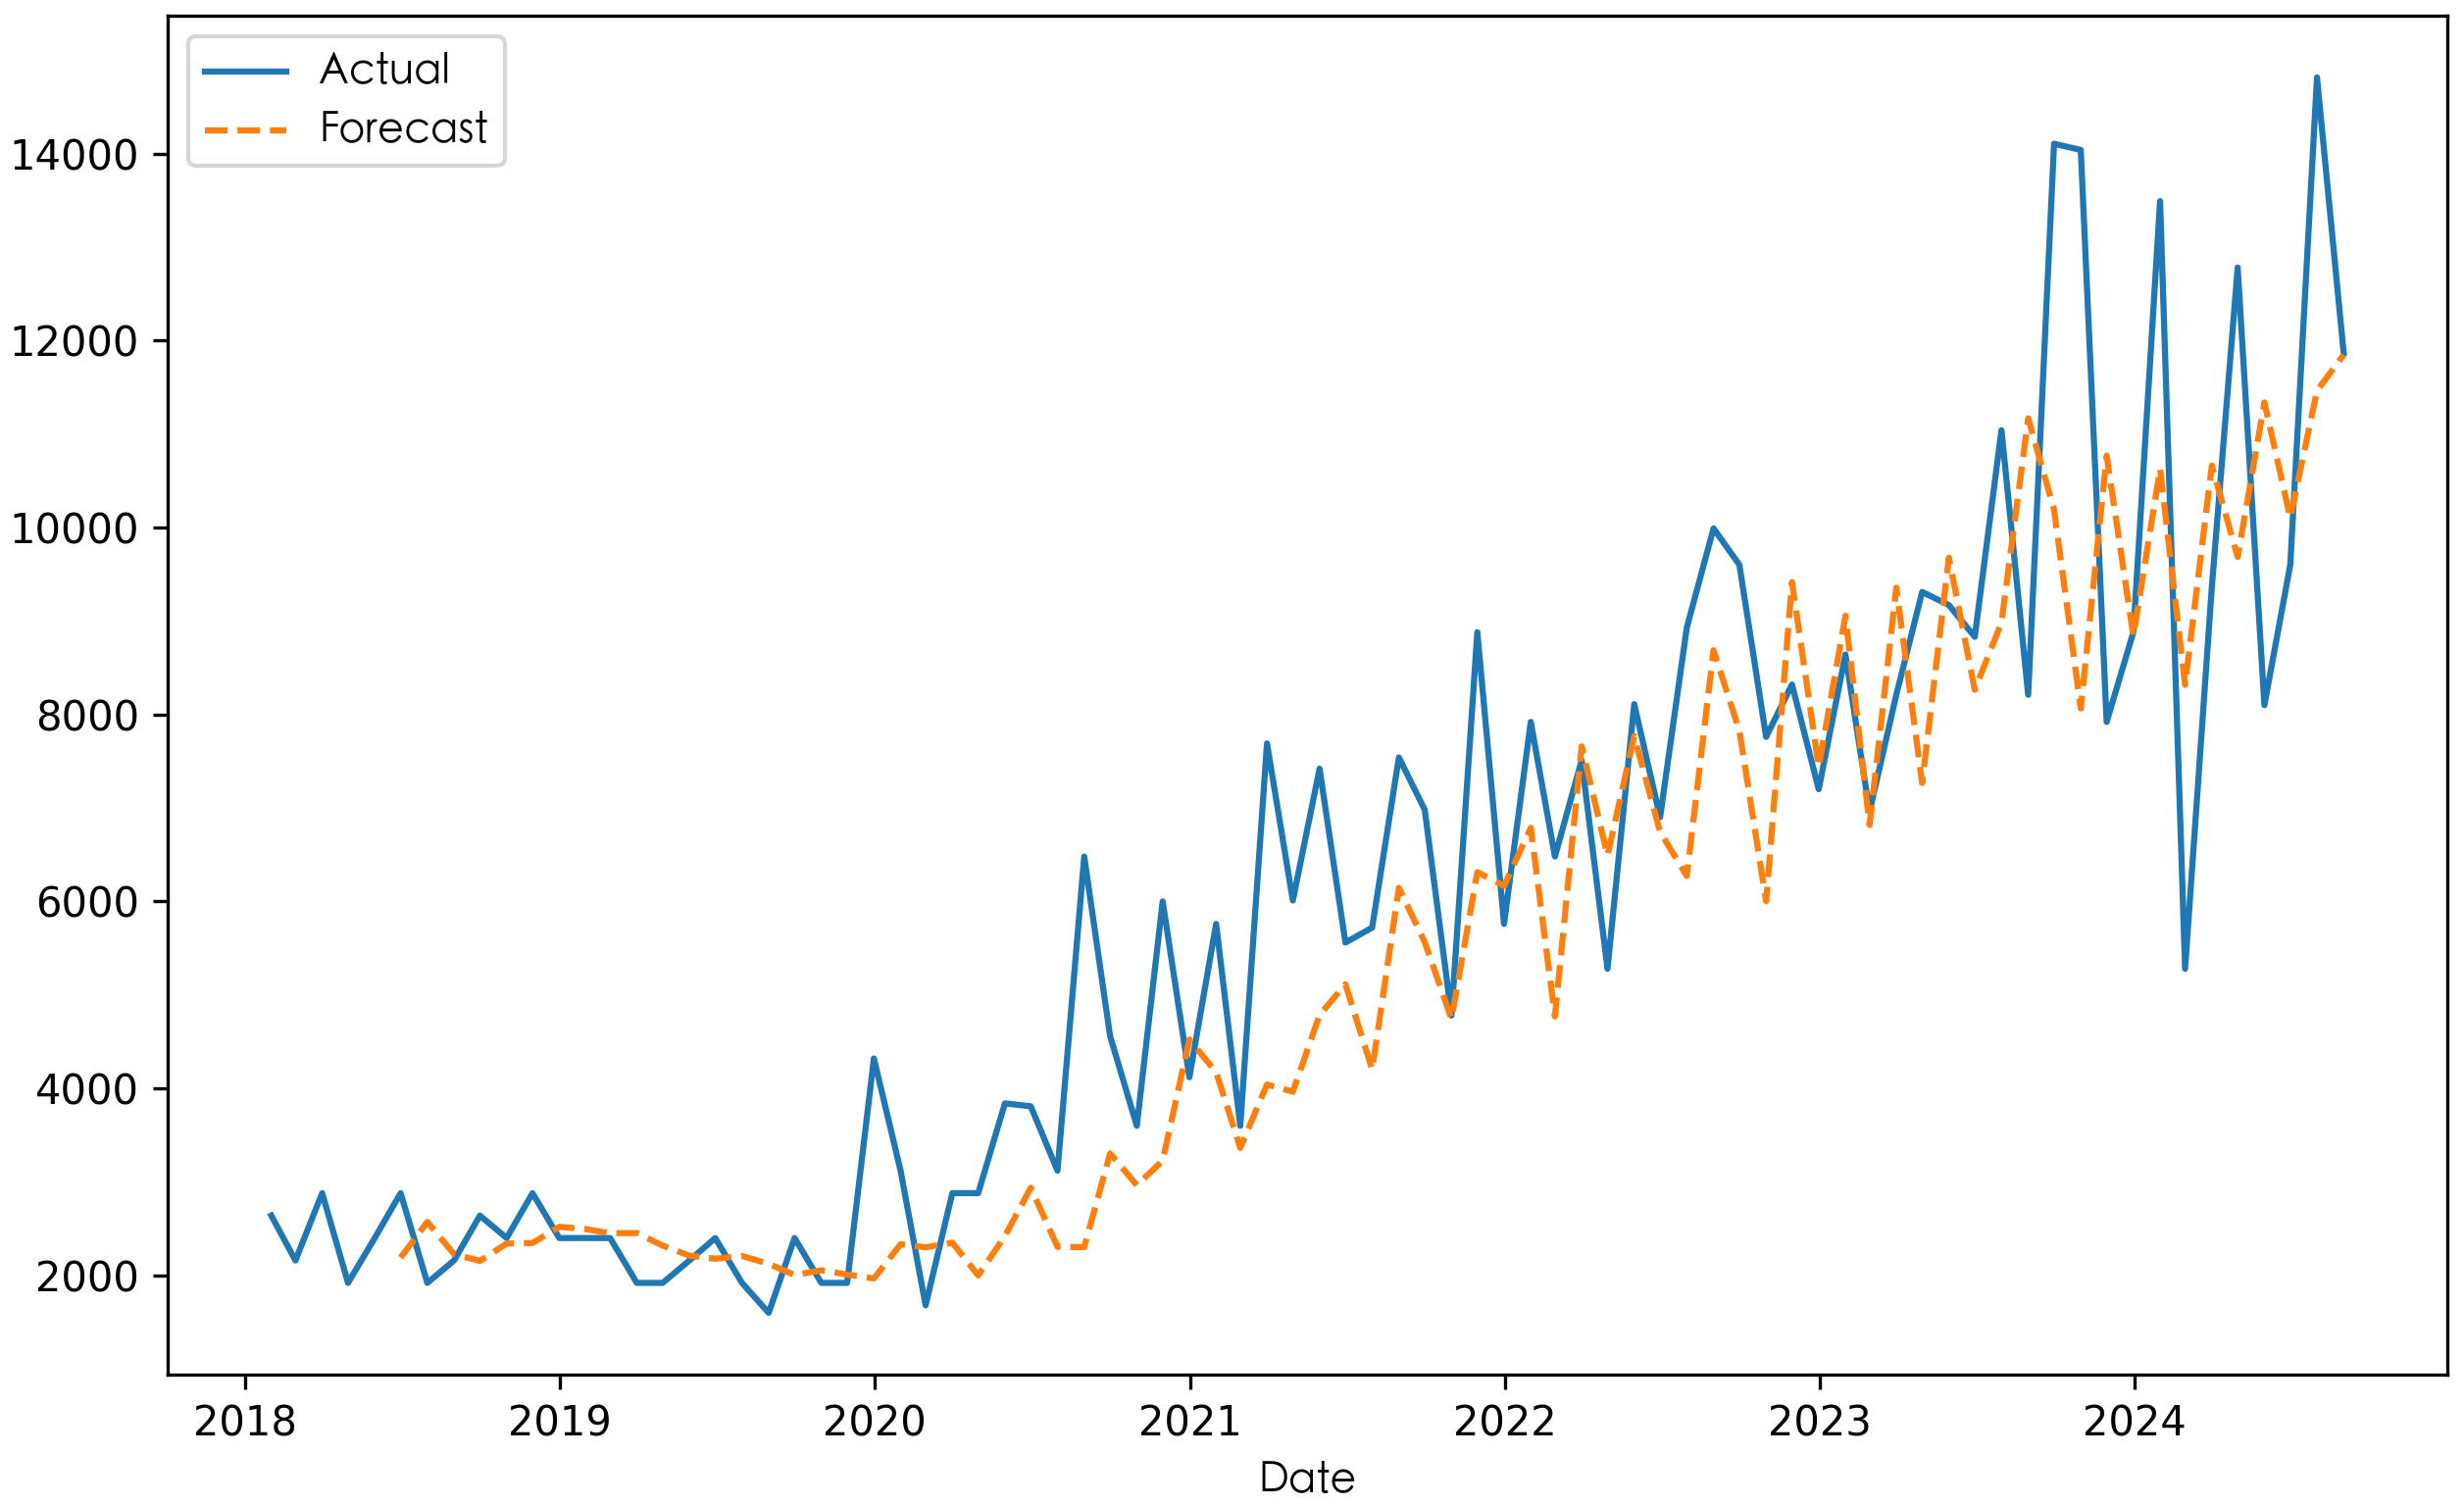
\includegraphics[width=\linewidth]{../Result_Paper/Prophet_Prediction_肾衰宁片_山海关药业.png}
\caption{Prophet Prediction for Shenshuaining Tablets by Shanhaiguan Pharmaceutical.}
\label{fig:shenshuaining}
\end{figure}
\end{itemize}

\paragraph{DynamicXSP-S (SARIMAX) Model}
\begin{itemize}
\item \textbf{Drug:} Peritoneal Dialysis Solution [Lactate]
\begin{itemize}
\item \textbf{Manufacturer:} Huaren
\item \textbf{Metrics:} $R^2 = 0.8109$, SMAPE = 32.49
\end{itemize}
SARIMAX demonstrated superior performance for this drug due to its ability to capture both the seasonal patterns and the gradual decline in demand shown in the time series. The model effectively handled the relatively stable periodic fluctuations until the sharp decline in 2023.
\begin{figure}[H]
\centering
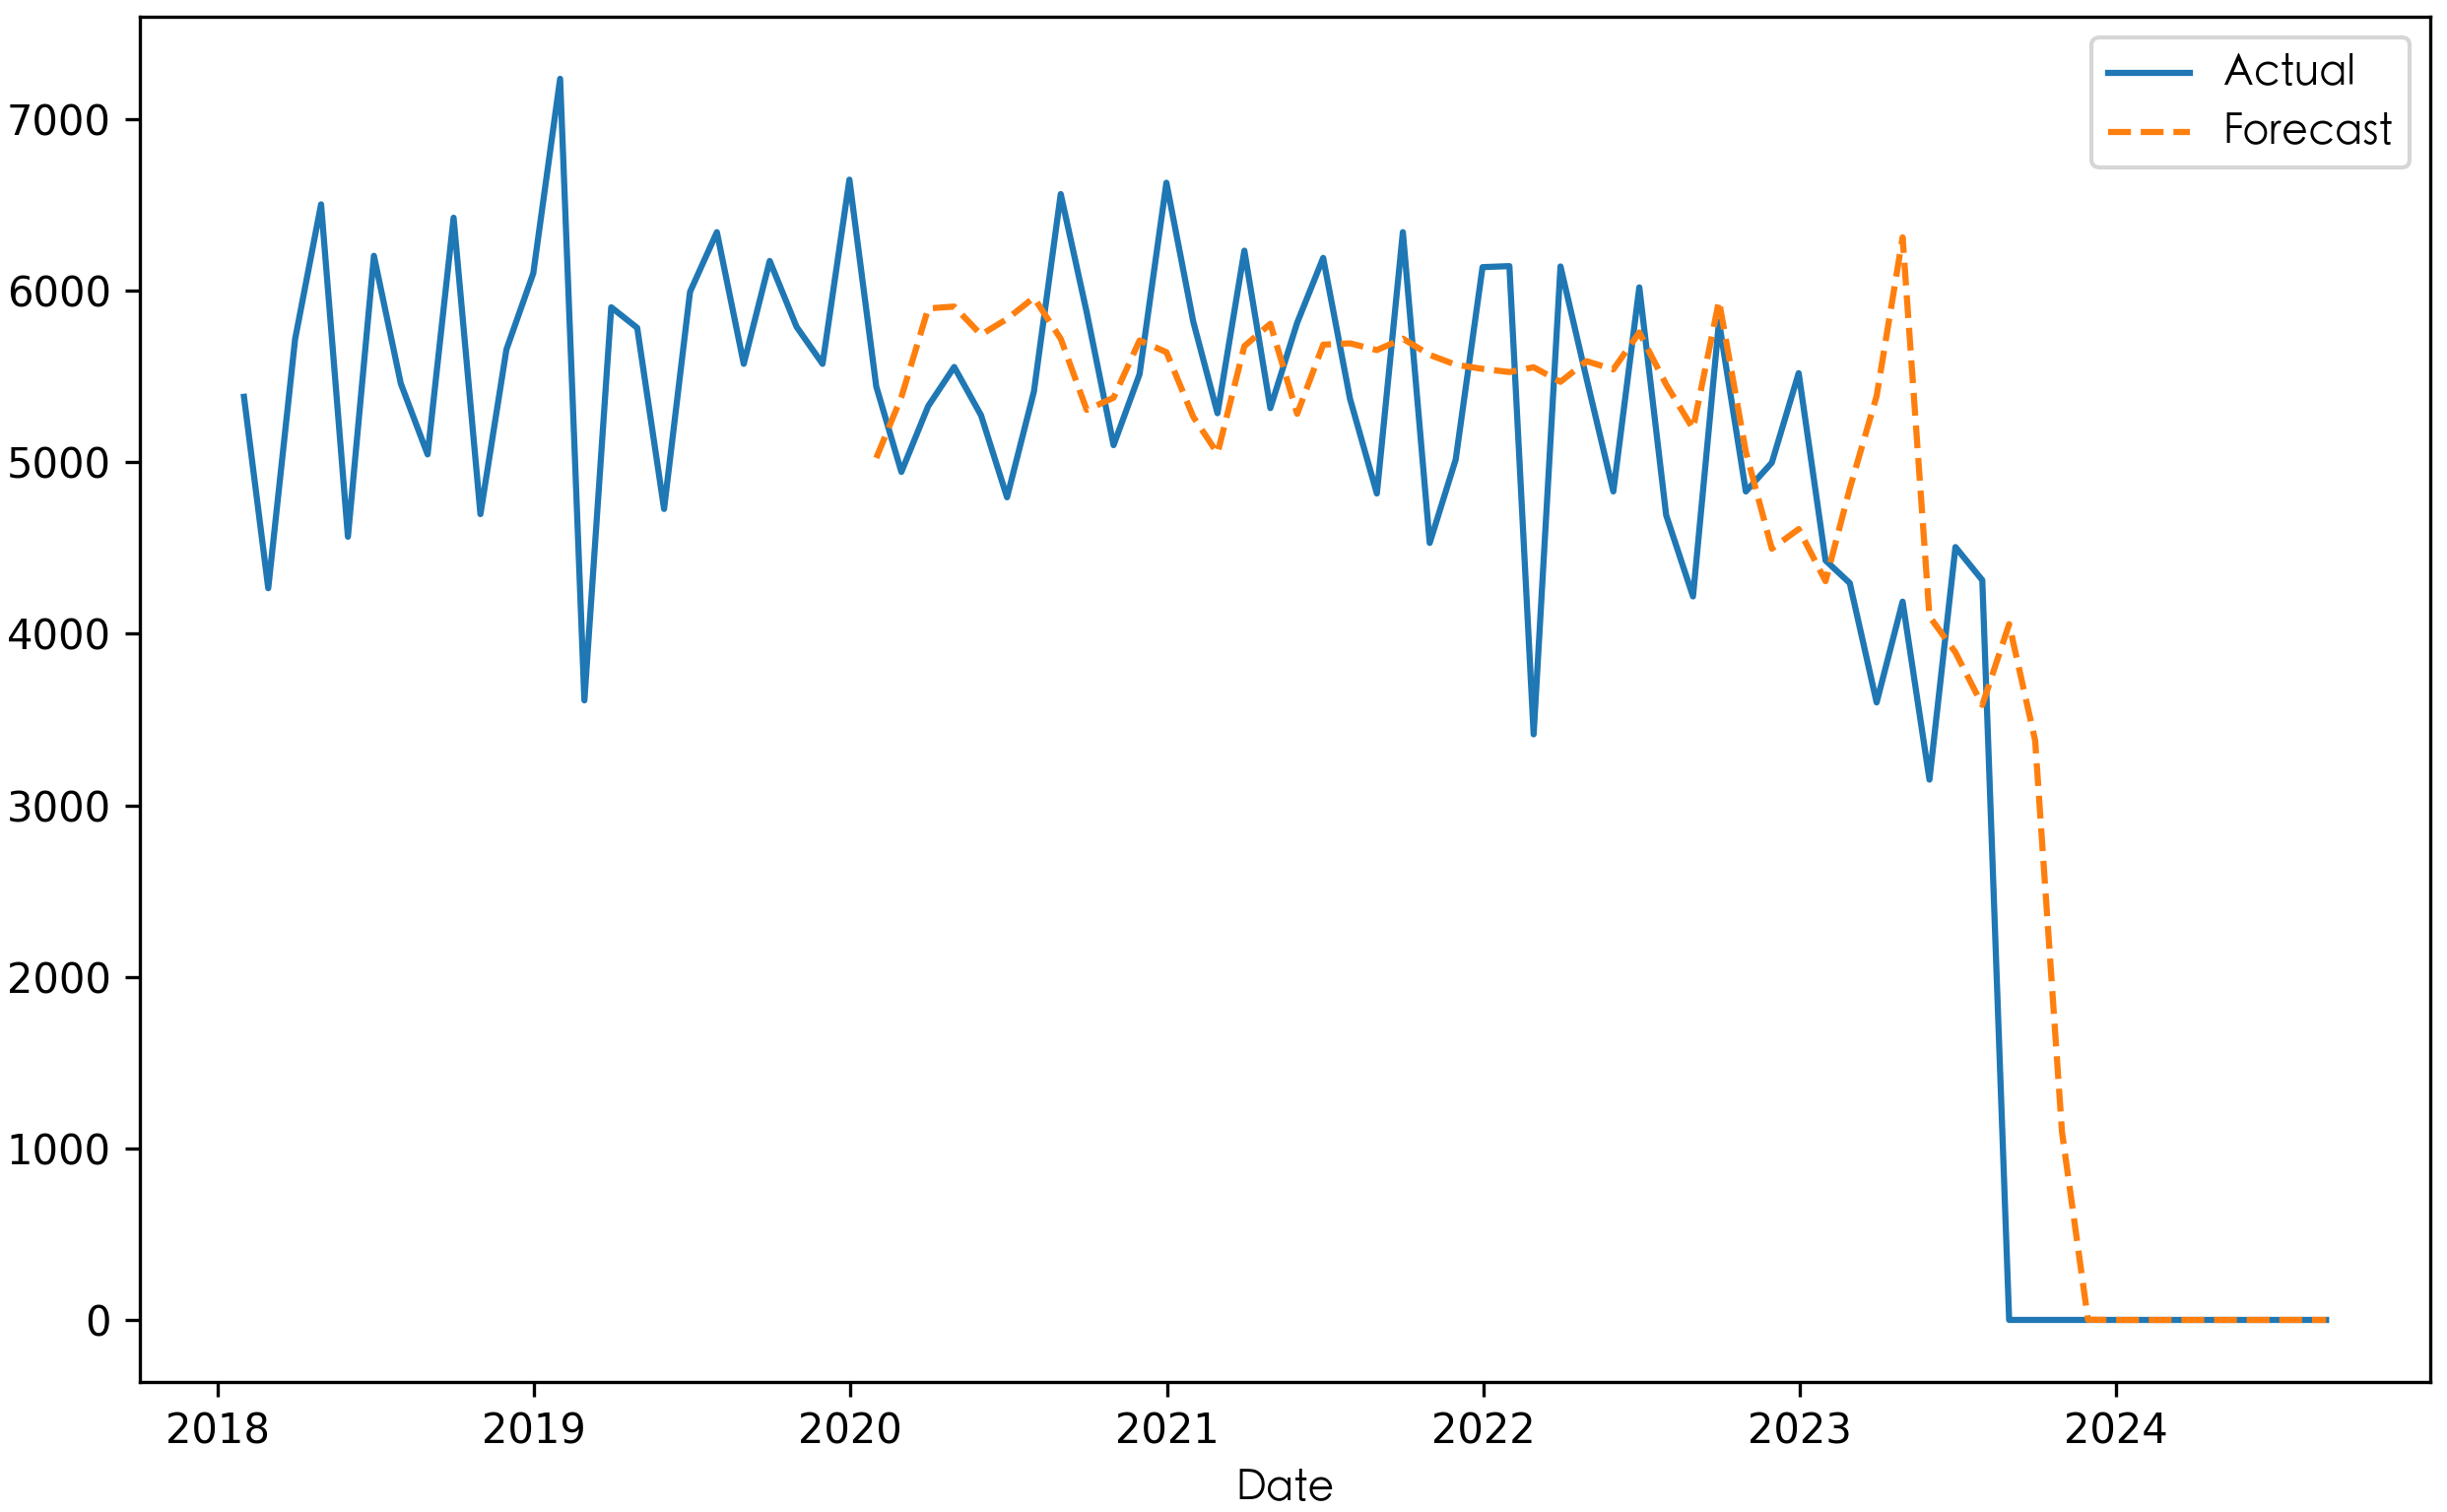
\includegraphics[width=\linewidth]{../Result_Paper/SARIMAX_Prediction_腹膜透析液[乳酸盐]_华仁.png}
\caption{SARIMAX Prediction for Peritoneal Dialysis Solution by Huaren.}
\label{fig:peritoneal}
\end{figure}
\item \textbf{Drug:} Vitamin B1 Tablets
\begin{itemize}
\item \textbf{Manufacturer:} Xinyi Huanghe
\item \textbf{Metrics:} $R^2 = 0.7345$, SMAPE = 35.37
\end{itemize}
The SARIMAX model was effective for this drug due to its ability to handle the external influences and volatility in the sales data.
\begin{figure}[H]
\centering
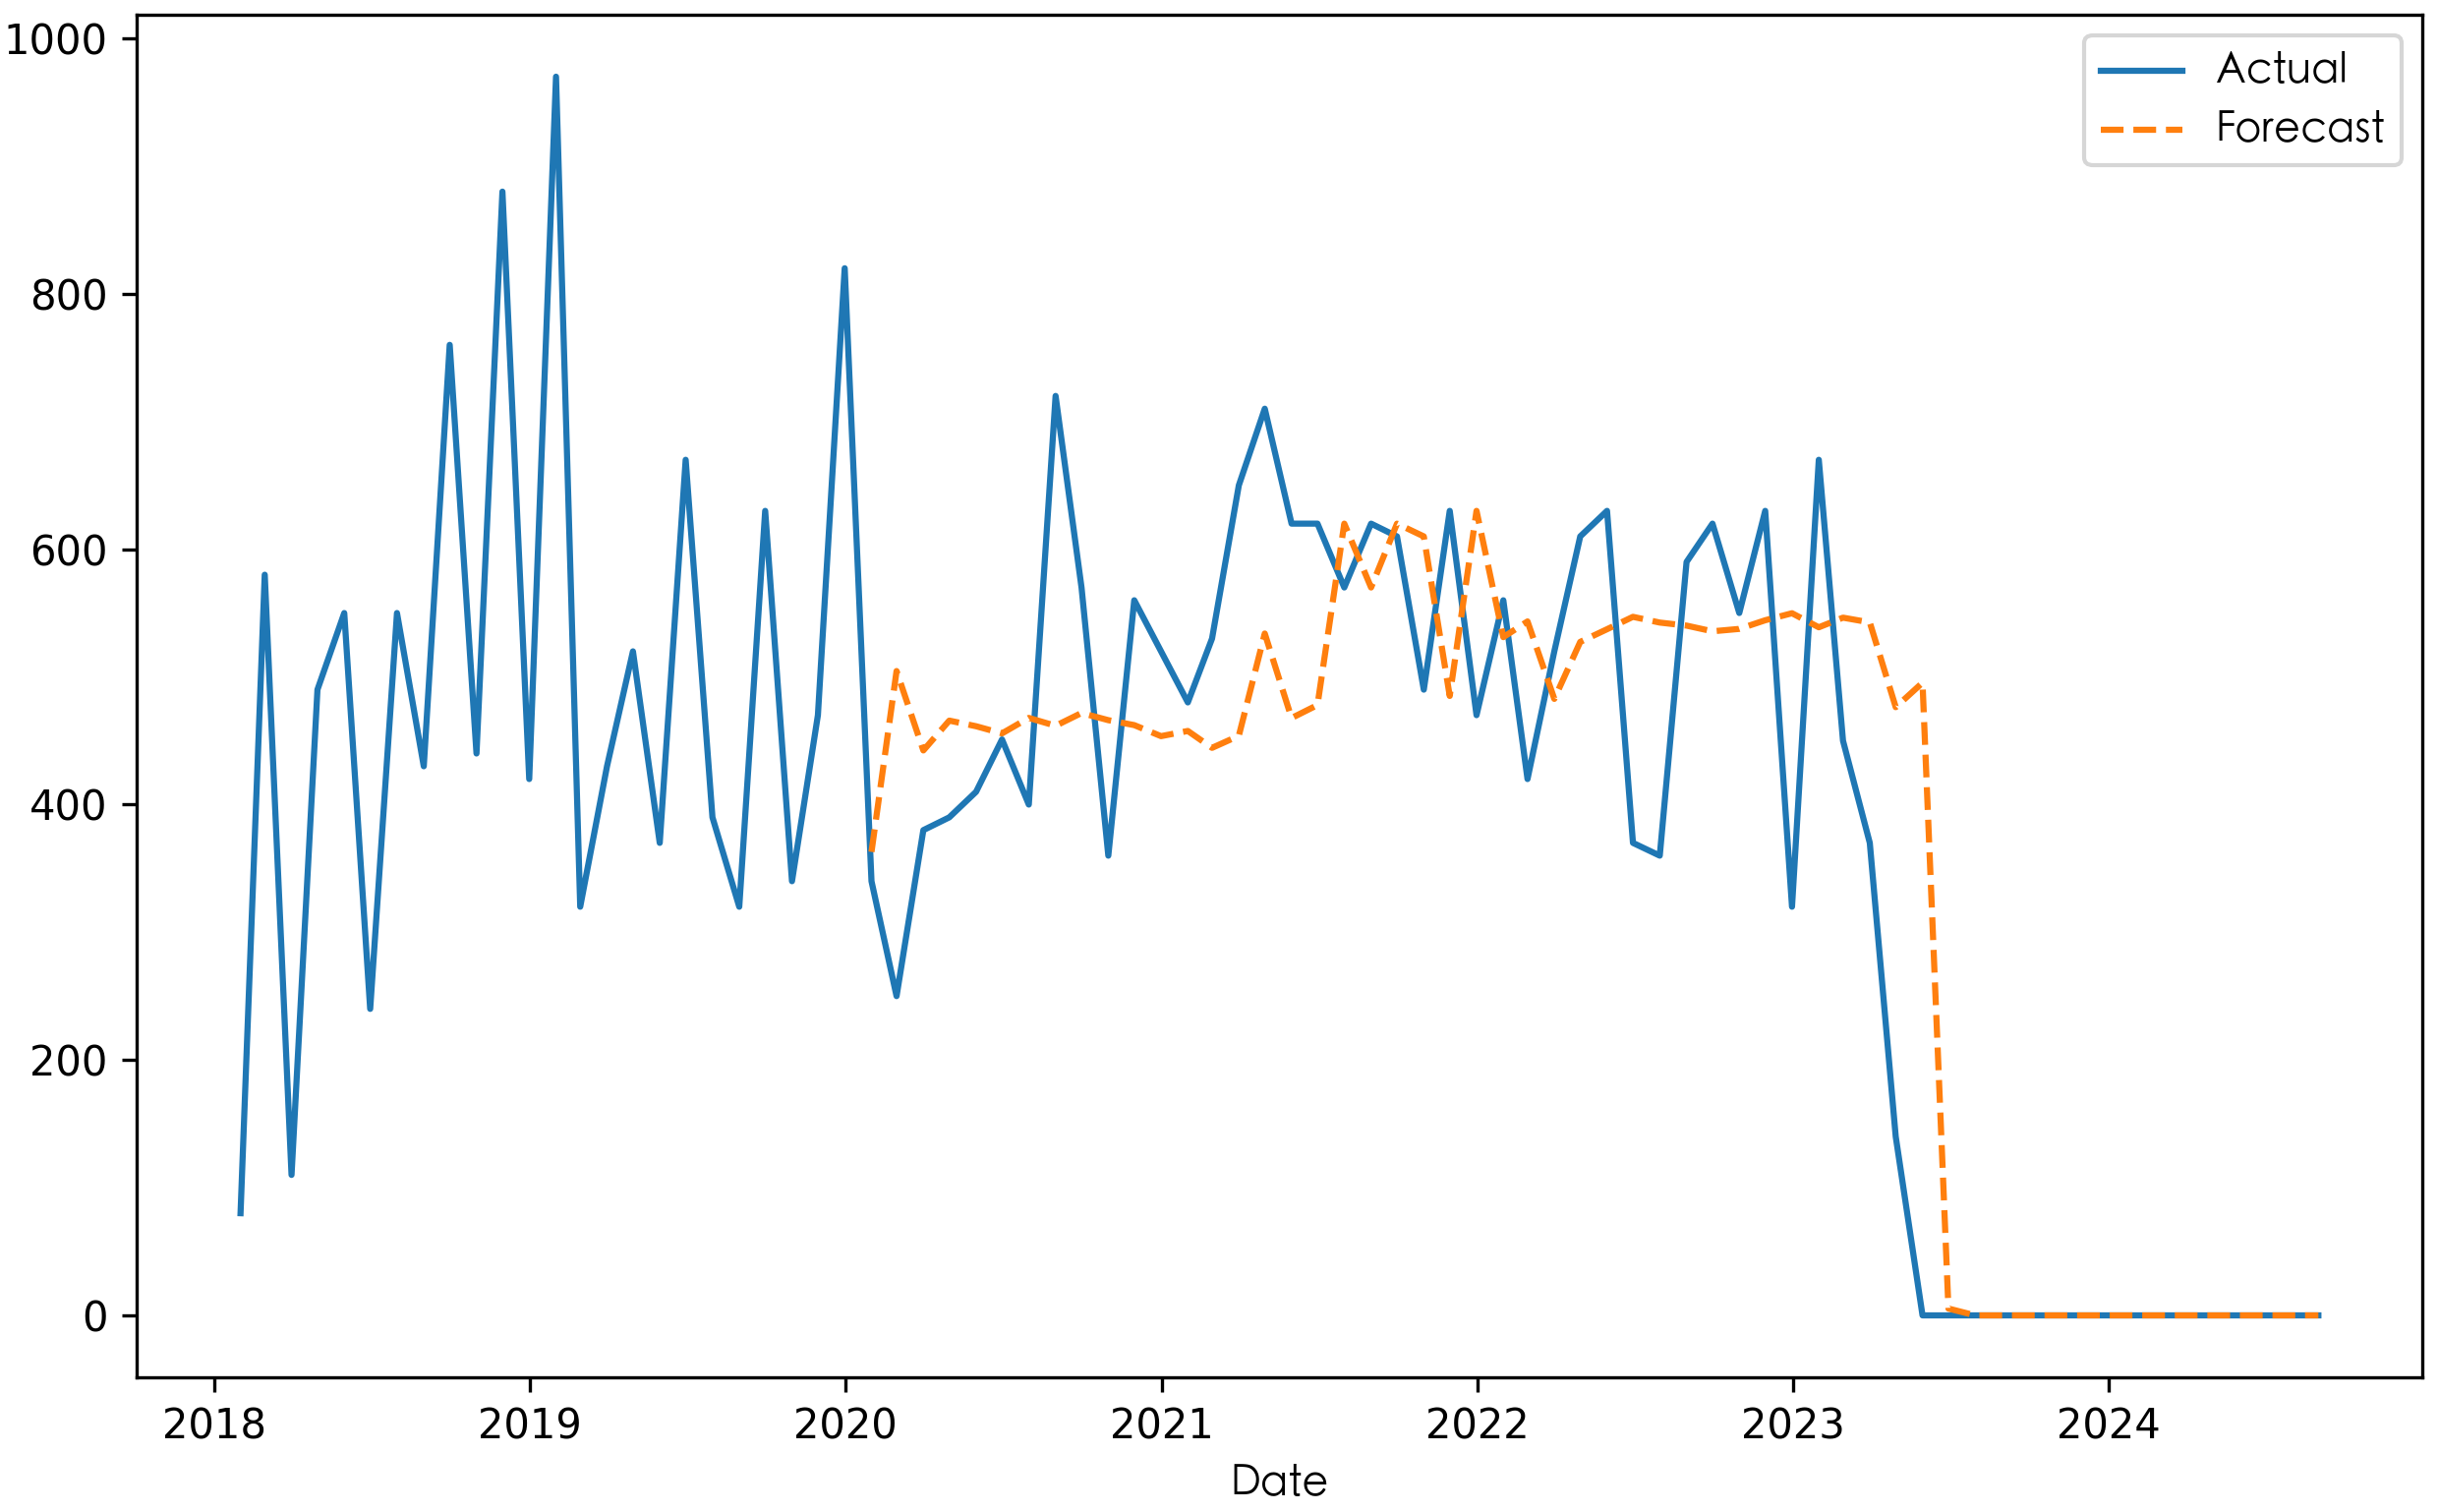
\includegraphics[width=\linewidth]{../Result_Paper/SARIMAX_Prediction_维生素B1片_信谊黄河.png}
\caption{SARIMAX Prediction for Vitamin B1 Tablets by Xinyi Huanghe.}
\label{fig:vitaminb1}
\end{figure}
\end{itemize}

\subsubsection{Overall Results}

The results highlighted that no single model universally outperformed the others across all cases, underscoring the importance of tailoring the choice of forecasting models to specific data characteristics. SARIMAX demonstrated superior capability in capturing seasonality influenced by external variables, such as pricing trends and policy changes. XGBoost excelled in modeling complex, non-linear relationships within the data, making it particularly effective for patterns with high variability. Prophet performed well in cases with dominant seasonality and long-term trends, such as periodic spikes in drug demand. These findings proves the necessary of DynamicXSP by leveraging the complementary strengths of each single model. 

The visualization analysis reveals several key findings:

\textbf{Long-term Trend Capture}:
\begin{itemize}
\item All models effectively captured the underlying growth trends, with Prophet showing particular strength in long-term pattern recognition.
\item SARIMAX demonstrated superior performance in capturing gradual trend changes, as evidenced in the insulin device forecasts.
\end{itemize}

\textbf{Seasonal Pattern Recognition}:
\begin{itemize}
\item XGBoost effectively captured complex seasonal patterns in chronic medication usage.
\item SARIMAX showed strong performance in regular seasonal variations, particularly in established products.
\end{itemize}

\textbf{Growth Pattern Adaptation}:
\begin{itemize}
\item Prophet demonstrated superior capability in adapting to emerging growth patterns.
\item XGBoost showed strong performance in capturing non-linear growth relationships.
\end{itemize}


\section{Conclusion and Future Work}

\subsection{Conclusion}

The results of this study underscore the effectiveness and adaptability of the DynamicXSP framework in addressing the challenges of pharmaceutical demand forecasting. By integrating the complementary strengths of SARIMAX, Prophet, and XGBoost, along with advanced techniques such as rolling-window forecasting, grid search and feature engineering, DynamicXSP provides a robust solution for predicting drug consumption across diverse drug-manufacturer combinations.

This framework's tailored approach allows the selection and integration of models based on the specific characteristics of each dataset, enabling it to overcome limitations inherent in single-model approaches. The performance evaluation highlights the key contributions of each model within the framework: 

\begin{itemize} 
    \item \textbf{DynamicXSP-X (XGBoost) Model}: Demonstrated superior handling of nonlinear relationships, particularly excelling in short-term predictions, where it outperformed SARIMAX and Prophet in terms of RMSE and SMAPE. 
    \item \textbf{DynamicXSP-S (SARIMAX) Model}: Excelled in datasets dominated by seasonal trends and where external (exogenous) variables, such as pricing or policy changes, played a significant role. 
    \item \textbf{DynamicXSP-P (Prophet) Model}: Effectively captured long-term seasonality and trends, proving valuable for datasets with prominent periodic patterns, though it faced challenges with sparsity. \end{itemize}

The DynamicXSP framework's ability to dynamically adapt to various data characteristics and leverage the complementary strengths of multiple models highlights its practicality and scalability for hospital pharmacy forecasting. This hybrid approach not only improves prediction accuracy and robustness but also sets a foundation for broader applications in healthcare demand forecasting.

\subsection{Future Work}
To further improve drug inventory predictions, the following directions are proposed for future research:

\begin{itemize}
    \item \textbf{Hybrid Framework Expansion}: Extend the hybrid framework by integrating additional models, such as LightGBM, Transformer-based architectures, or ensemble methods to capture both short-term fluctuations and long-term trends.
    \item \textbf{External Variable Enrichment}: Explore additional exogenous variables such as patient inflow, epidemic outbreak data, seasonal illnesses (e.g., flu seasons), or hospital-specific factors to improve prediction accuracy.
    \item \textbf{Automated Model Selection}: Implement automated hyperparameter tuning and model selection techniques (e.g., Bayesian optimization) to improve forecasting performance with minimal manual intervention.
\end{itemize}

By addressing these areas, the proposed framework can become a more robust and scalable solution for hospital pharmacy inventory management, ensuring operational efficiencies of hospital pharmacies.

\section{References}

\begin{thebibliography}{99}

    \bibitem{koala2021factors} 
    D. Koala, Z. Yahouni, G. Alpan, and Y. Frein, “Factors influencing drug consumption and prediction methods,” in \textit{CIGI-Qualita: Conférence Internationale Génie Industriel QUALITA}, Grenoble, France, 2021.
    
    \bibitem{taylor2018forecasting}
    S. J. Taylor and B. Letham, “Forecasting at scale,” \textit{The American Statistician}, vol. 72, no. 1, pp. 37–45, 2018.

    \bibitem{chen2016xgboost}
    T. Chen and C. Guestrin, “XGBoost: A scalable tree boosting system,” \textit{Proceedings of the 22nd ACM SIGKDD International Conference on Knowledge Discovery and Data Mining}, 2016, pp. 785–794.

    \bibitem{meng2021comparative}
    J. Meng, Q. Zhang, and X. Li, “Comparative analysis of Prophet and LSTM models in drug sales forecasting,” \textit{Journal of Physics: Conference Series}, vol. 1910, no. 1, p. 012059, 2021.

    \bibitem{xu2019hybrid}
    W. Xu, Y. Wang, and J. Zhao, “A hybrid modelling method for time series forecasting based on a linear regression model and deep learning,” \textit{Applied Intelligence}, vol. 49, no. 7, pp. 2875–2888, 2019.

    \bibitem{siddiqui2021hybrid}
    R. Siddiqui, A. Khan, and M. Ahmed, “A Hybrid Demand Forecasting Model for Greater Forecasting Accuracy: The Case of the Pharmaceutical Industry,” \textit{Supply Chain Forum: An International Journal}, vol. 22, no. 3, pp. 1–13, 2021.

    \bibitem{rathipriya2022pharma}
    R. Rathipriya, M. Saranya, and K. Ramkumar, “Demand Forecasting Model for Time-Series Pharmaceutical Data Using Neural Networks,” \textit{Neural Computing and Applications}, vol. 35, pp. 1945–1957, 2022.

\end{thebibliography}

\appendix
\section{Sample Selection Algorithm}
\label{appendix:sample-selection}

The following pseudocode outlines the sample selection process used to ensure the quality and relevance of the dataset for modeling tasks:

\begin{algorithm}[H]
\caption{Sample Selection Algorithm}
\begin{algorithmic}[1]
\Require Cleaned data $df$, configuration thresholds $\text{config}$
\Ensure Filtered dataset $final\_df$
\State $final\_df \gets \emptyset$
\For{each unique combination of drug name and manufacturer $(d, m)$ in $df$}
    \State $group\_data \gets$ subset of $df$ for $(d, m)$
    \If{length of $group\_data < \text{config.min\_months}$ \textbf{or} sum of consumption $= 0$}
        \State \textbf{Skip group} \Comment{Insufficient or sparse data}
    \EndIf
    \State $non\_zero\_ratio \gets$ proportion of non-zero consumption in $group\_data$
    \If{$non\_zero\_ratio < \text{config.sparsity\_threshold}$}
        \State \textbf{Skip group} \Comment{Data too sparse}
    \EndIf
    \State $acf\_values \gets$ autocorrelation function of consumption in $group\_data$
    \If{$\max(acf\_values[1:]) < \text{config.min\_acf\_threshold}$}
        \State \textbf{Skip group} \Comment{Insufficient autocorrelation}
    \EndIf
    \If{no start date $\geq \text{config.min\_start\_date}$ in $group\_data$}
        \State \textbf{Skip group} \Comment{No recent data}
    \EndIf
    \State $variance \gets$ variance of consumption in $group\_data$
    \If{$variance < \text{config.min\_variance\_threshold}$}
        \State \textbf{Skip group} \Comment{Variance too low}
    \EndIf
    \State $missing\_ratio \gets$ maximum missing ratio for features in $group\_data$
    \If{$missing\_ratio > \text{config.max\_missing\_ratio}$}
        \State \textbf{Skip group} \Comment{Feature missing data too high}
    \EndIf
    \State $skewness \gets$ skewness of consumption in $group\_data$
    \If{$|skewness| > \text{config.max\_skewness}$}
        \State \textbf{Skip group} \Comment{Target variable too skewed}
    \EndIf
    \State $correlation \gets$ correlation of consumption with lagged features in $group\_data$
    \If{$|correlation| < \text{config.min\_correlation}$}
        \State \textbf{Skip group} \Comment{Insufficient correlation with features}
    \EndIf
    \State $final\_df \gets final\_df \cup group\_data$
\EndFor
\State \Return $final\_df$
\end{algorithmic}
\end{algorithm}

\bibliographystyle{IEEEtran}
\bibliography{references}

\end{document}
